\documentclass[conference]{IEEEtran}
\usepackage{amsmath,amssymb,amsthm,booktabs,graphicx,hyperref}

\title{The Observation--Action Safety Gap: A Quantitative Signature with Battery and AV Witness Domains}
\author{Pratik Niroula}

\begin{document}
\maketitle

\begin{abstract}
The Observation--Action Safety Gap (OASG) describes the release-time mismatch in which a controller evaluates safety on a degraded observation even though the true physical state has already left the safe set. This paper makes that phenomenon measurable with a scalar signature computed from logged trajectories. The defended quantitative scope is intentionally narrow: only the Battery and autonomous-vehicle witness domains are treated as numeric evidence in the current submission package. The resulting metric is operational rather than universal, but it is precise enough to support falsifiable comparisons across replay traces and runtime monitors.
\end{abstract}

\section{Introduction}
Safety failures in cyber-physical systems often arise from an information mismatch rather than a complete control collapse. The controller continues to act coherently on the observation channel, yet the physical state has already crossed the boundary that the release decision was supposed to protect. ORIUS names that release-time mismatch the Observation--Action Safety Gap. The framing is adjacent to runtime assurance, fault detection, and cyber-physical monitoring, but it is not identical to any one of those literatures \cite{sha1998simplex,sha2001using,pasqualetti2013attack,basseville1993detection}.

Naming the phenomenon is not enough for submission-quality evidence. A reviewer should be able to inspect a metric definition, compare it to the code, and recompute it from logged trajectories. This paper therefore focuses on a bounded quantitative object rather than a universal plant law.

\section{Definition}
Let $x_t$ denote the true state, $o_t$ the observed state, $\mathcal{C}$ the safe set, and $w_t \in [0,1]$ a runtime reliability score. The canonical gap event is
\[
\mathrm{gap}_t := (o_t \in \mathcal{C}) \wedge (x_t \notin \mathcal{C}) \wedge (w_t < 1).
\]
The canonical OASG signature is the weighted mean
\[
\Sigma_{\mathrm{OASG}} = \mathbb{E}_t \left[d(x_t,\mathcal{C})^+ \cdot \mathbf{1}[\mathrm{gap}_t]\right].
\]
Two auxiliary quantities make the signature interpretable:
\[
\rho_{\mathrm{exp}} = \mathbb{E}_t[\mathbf{1}[\mathrm{gap}_t]],
\qquad
s_{\mathrm{sev}} = \mathbb{E}_t[d(x_t,\mathcal{C})^+ \mid \mathrm{gap}_t].
\]
Whenever the gap event has positive probability, the invariant
\[
\Sigma_{\mathrm{OASG}} = \rho_{\mathrm{exp}} \cdot s_{\mathrm{sev}}
\]
holds by construction. Blindness is retained only as an auxiliary diagnostic describing how much of the true-unsafe surface is missed by the observation-facing check; it is not part of the primary signature formula.

\section{Computation Protocol}
The implementation consumes true states, observations, reliability scores, a safe-set test, and a signed distance-to-boundary function. Per-step contributions are $d(x_t,\mathcal{C})^+ \mathbf{1}[\mathrm{gap}_t]$, and the reported scalar is the sample mean of those contributions. Confidence intervals are estimated with a nonparametric bootstrap.

The current submission scope is Battery + AV only. Healthcare, industrial, navigation, and aerospace remain architecture or future-work surfaces in the broader repository, but they are intentionally excluded from defended quantitative tables here because the submission branch does not treat them as locked witness artifacts.

\IfFileExists{signature_table.tex}{
\begin{table}[t]
\centering
\caption{Battery + AV OASG signatures computed from the canonical benchmark layer.}
\begin{tabular}{lrrrr}
\toprule
Domain & Signature & Exposure & Severity & Blindness \\
\midrule
Battery & 0.1033 & 0.055 & 1.8883 & 1.000 \\
Autonomous Vehicles & 73.0536 & 0.426 & 171.4512 & 0.681 \\
\bottomrule
\end{tabular}
\end{table}
}{}

\IfFileExists{signature_figure.pdf}{
\begin{figure}[t]
\centering
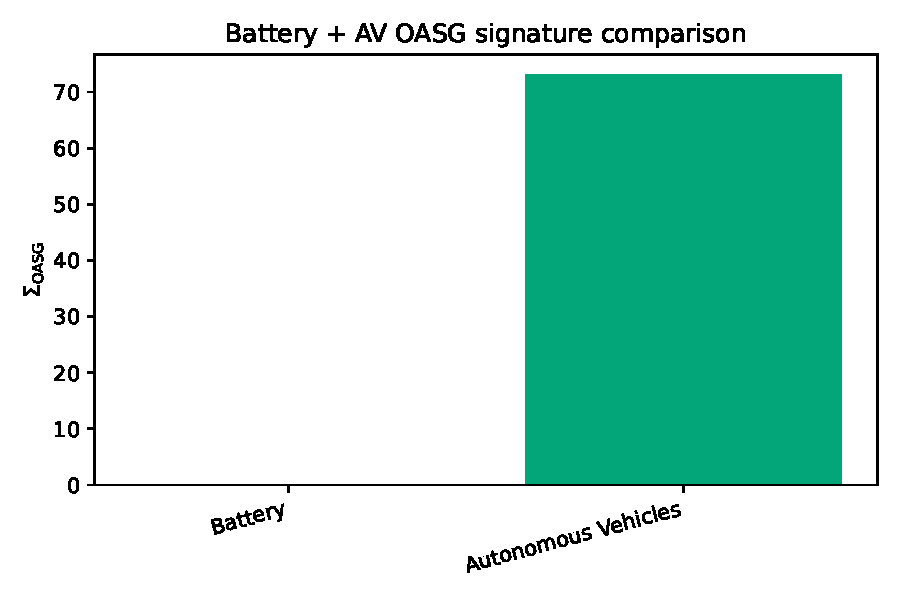
\includegraphics[width=\linewidth]{signature_figure.pdf}
\caption{Battery + AV OASG signature comparison.}
\end{figure}
}{}

\section{Interpretation}
The OASG signature does not replace runtime assurance, conformal calibration, or action repair. It measures the hidden true-state violation mass that those mechanisms must absorb. A larger signature can arise from more frequent gap events, more severe latent violations, or both, which is why exposure and severity are always reported alongside the scalar.

\section{Limitations}
This paper makes a bounded claim. It does not argue that one scalar captures all degraded-observation risk, and it does not present healthcare, industrial, navigation, or aerospace numbers as defended evidence. The contribution is a reproducible measurement protocol together with Battery and AV witness-domain measurements that can be checked against the code path in the benchmark layer.

\bibliographystyle{IEEEtran}
\bibliography{../refs}
\end{document}
